\chapter{Evaluation}

\section{Model Comparison}\label{inference}

Figure~\ref{rmse_bar} shows the root mean square error across all of the models.
Linear model serves as a baseline for comparison.
All of the neural network models improve upon the accuracy of the linear model, as is expected \cite{jeong2004bus}.

The MLP and CNN architectures achieve similar accuracy.
Both models fall under the class of feed forward models, meaning data is feed from input to output without any feedback loops.
However, the MLP model is symmetric about the inputs, meaning that no temporal aspects can be extracted from the input.
This is by nature of the network being fully connected, so each input is treated equally.
However in the case of the CNN, the model is not symmetric about the inputs.
Specifically, the 1D convolutions act in order on the input sequence.
In image processing, this ordering is used to capture translational invariance.
However for time series prediction, convolutions capture high level patterns in sequences which are then used as features for prediction in the fully connected layers.
This temporal aspect is possibly what gives the CNN advantage over the MLP.
Additionally the CNN is a larger model, with many more parameters than the MLP.
This increases the variance of the model and allows it to capture more patterns in the data.

\begin{figure}
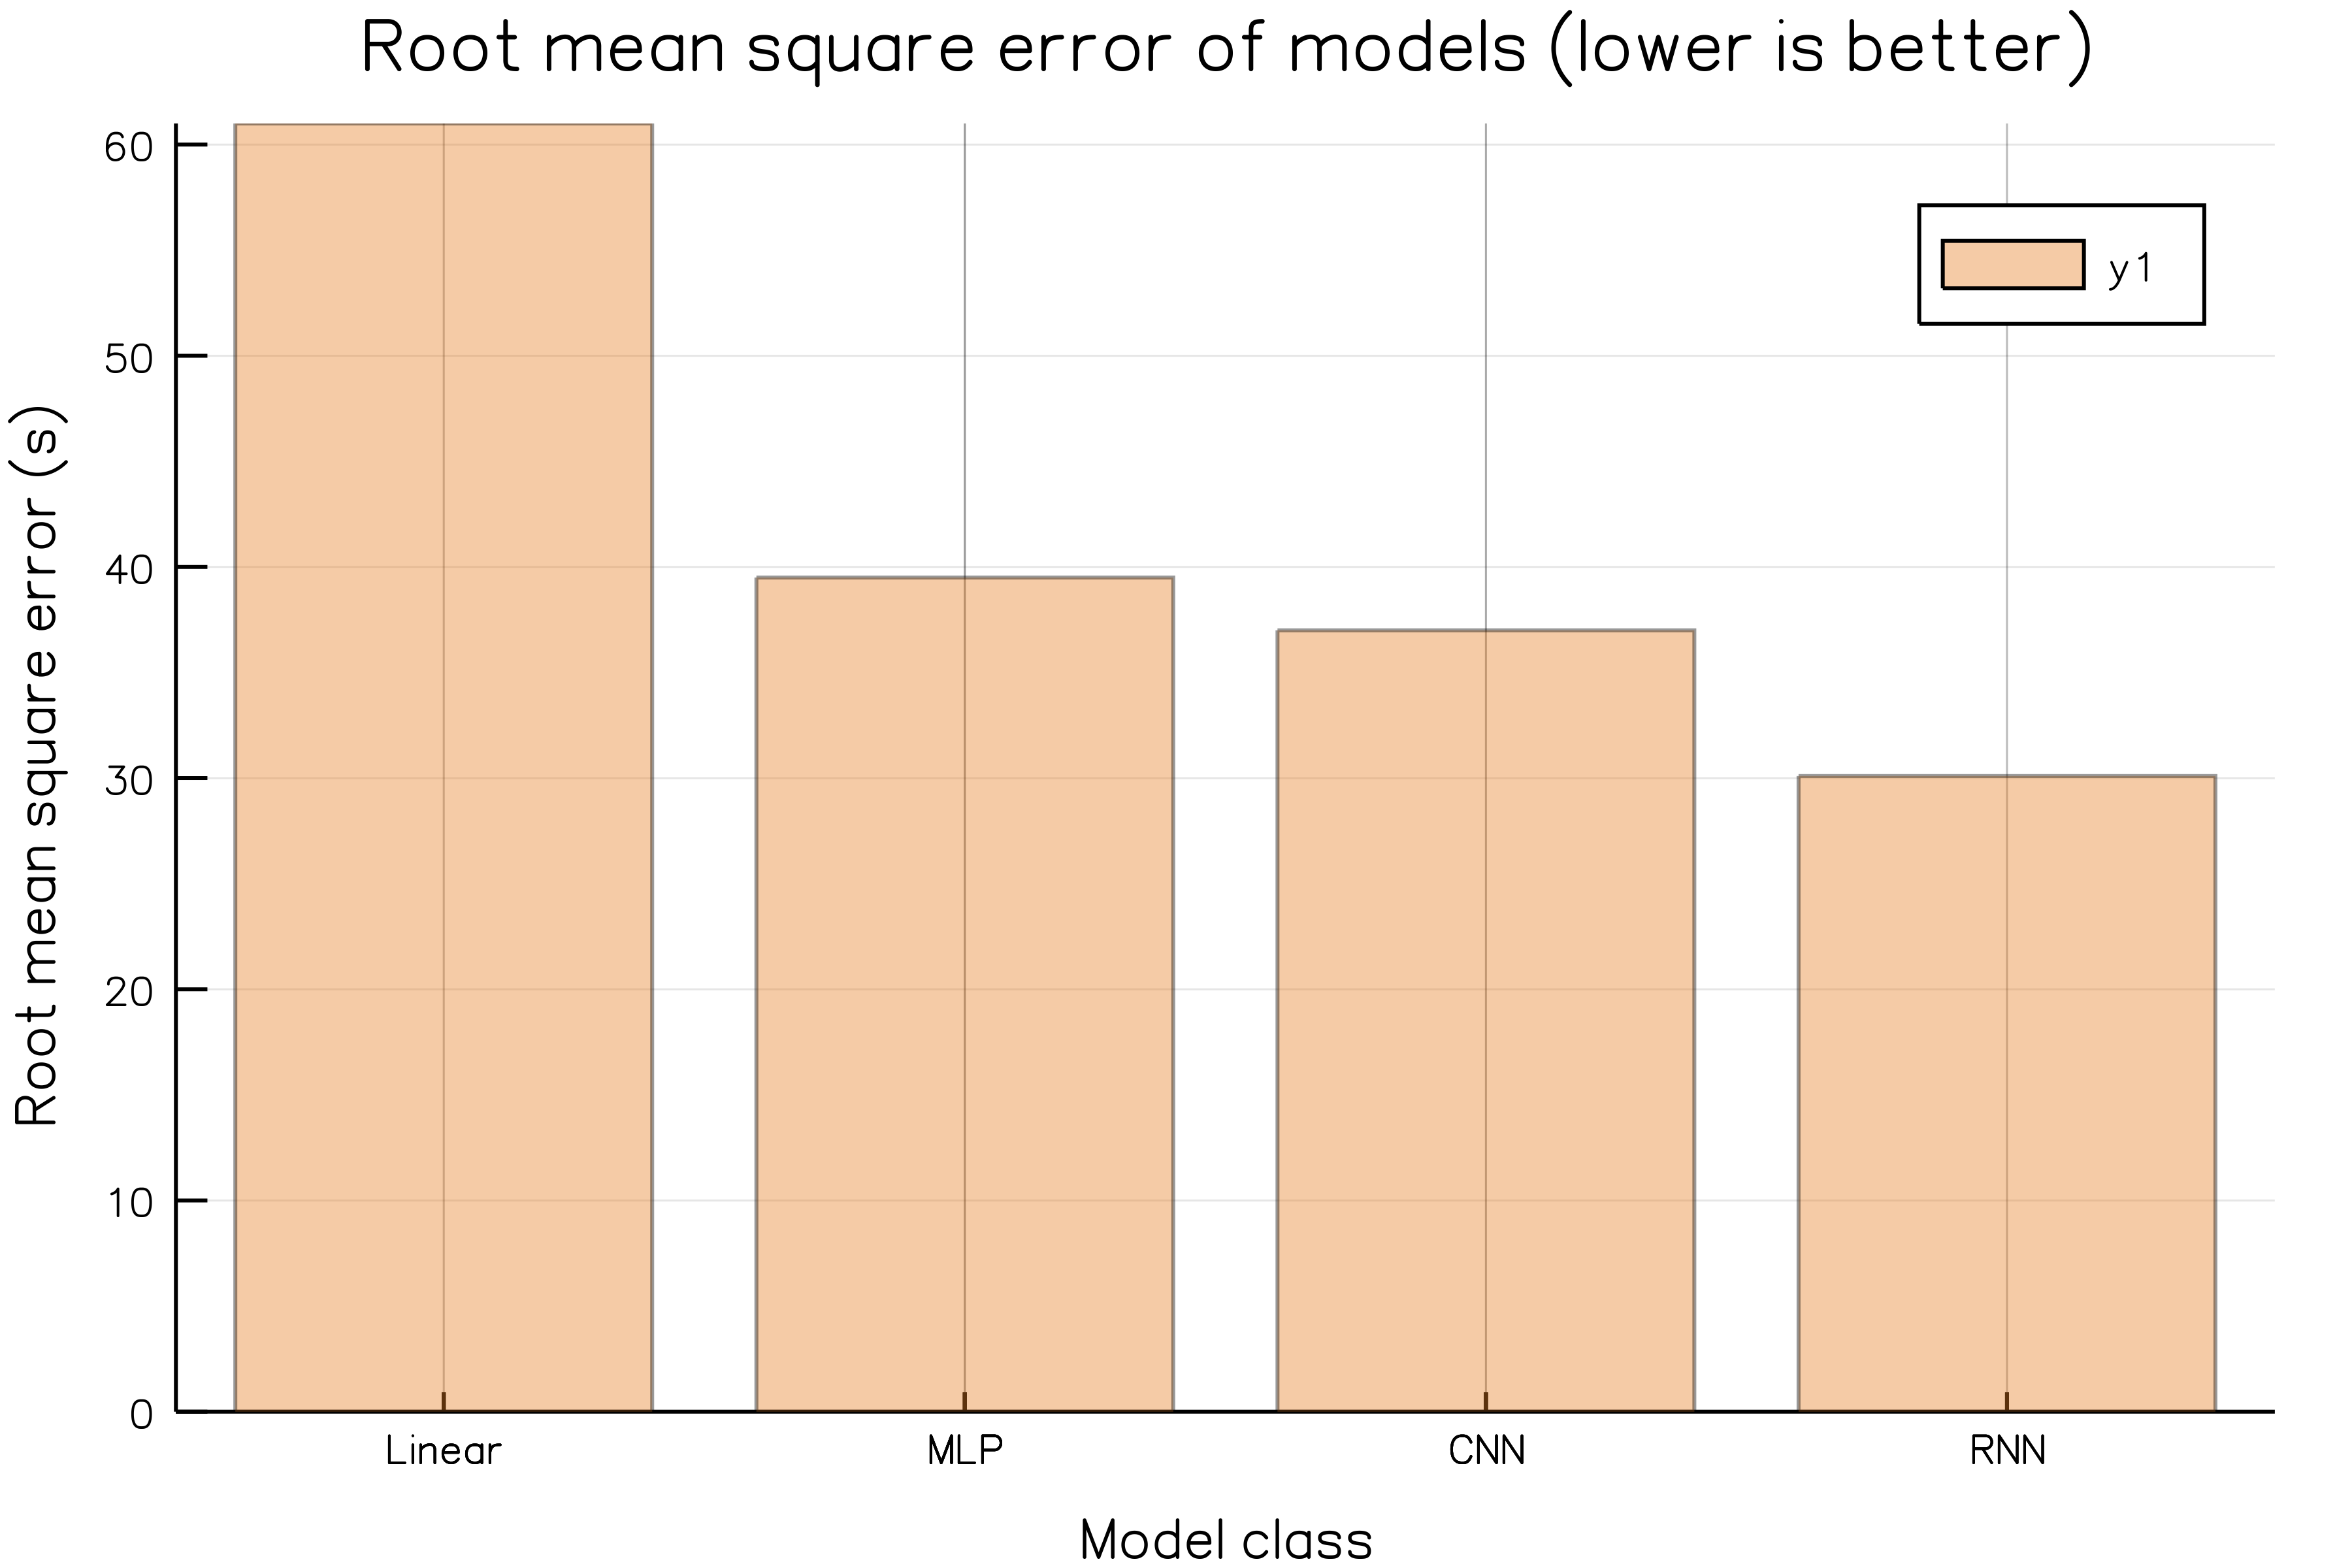
\includegraphics[width=\linewidth]{images/rmse_bar.png}
%\vspace{2.4in}
\caption{Root mean square error across all models}
\label{rmse_bar}
\end{figure}
\clearpage
\newpage

Figure~\ref{r2_bar} shows the coefficient of determination ($R^2$) score for each of the models.
The R squared score shows how much in the variance of the data the model is able to capture.
Zero indicates that the model is as good as random guessing, while a score of 1 indicates the model perfectly captures the data.
The linear model achieves an $R^2$ score of around 0.3.
This shows that the linear model does not do a great job of modeling the data, as is expected.
The linear model does not have enough expressivity to capture some of the more subtle patterns in the data.

The best coefficient of determination comes from the RNN, which achieves around 0.67.
This represents much better performance than the linear model.
However, there is still a lot of variance in the underlying data which the model cannot capture.
This gets back to the issue of the stochastic nature of traffic.
Large deviations can occur in traffic networks for various reasons which makes prediction difficult.
For example traffic accidents and construction are not included as features to the model, and these factors make a drastic impact on the underlying network.
To some extent, incorporating more data into the feature set will increase the amount of variance the model can capture.
However, this also requires increasing the size of the model, which may lead to overfitting, and decreased inference performance.

\begin{figure}
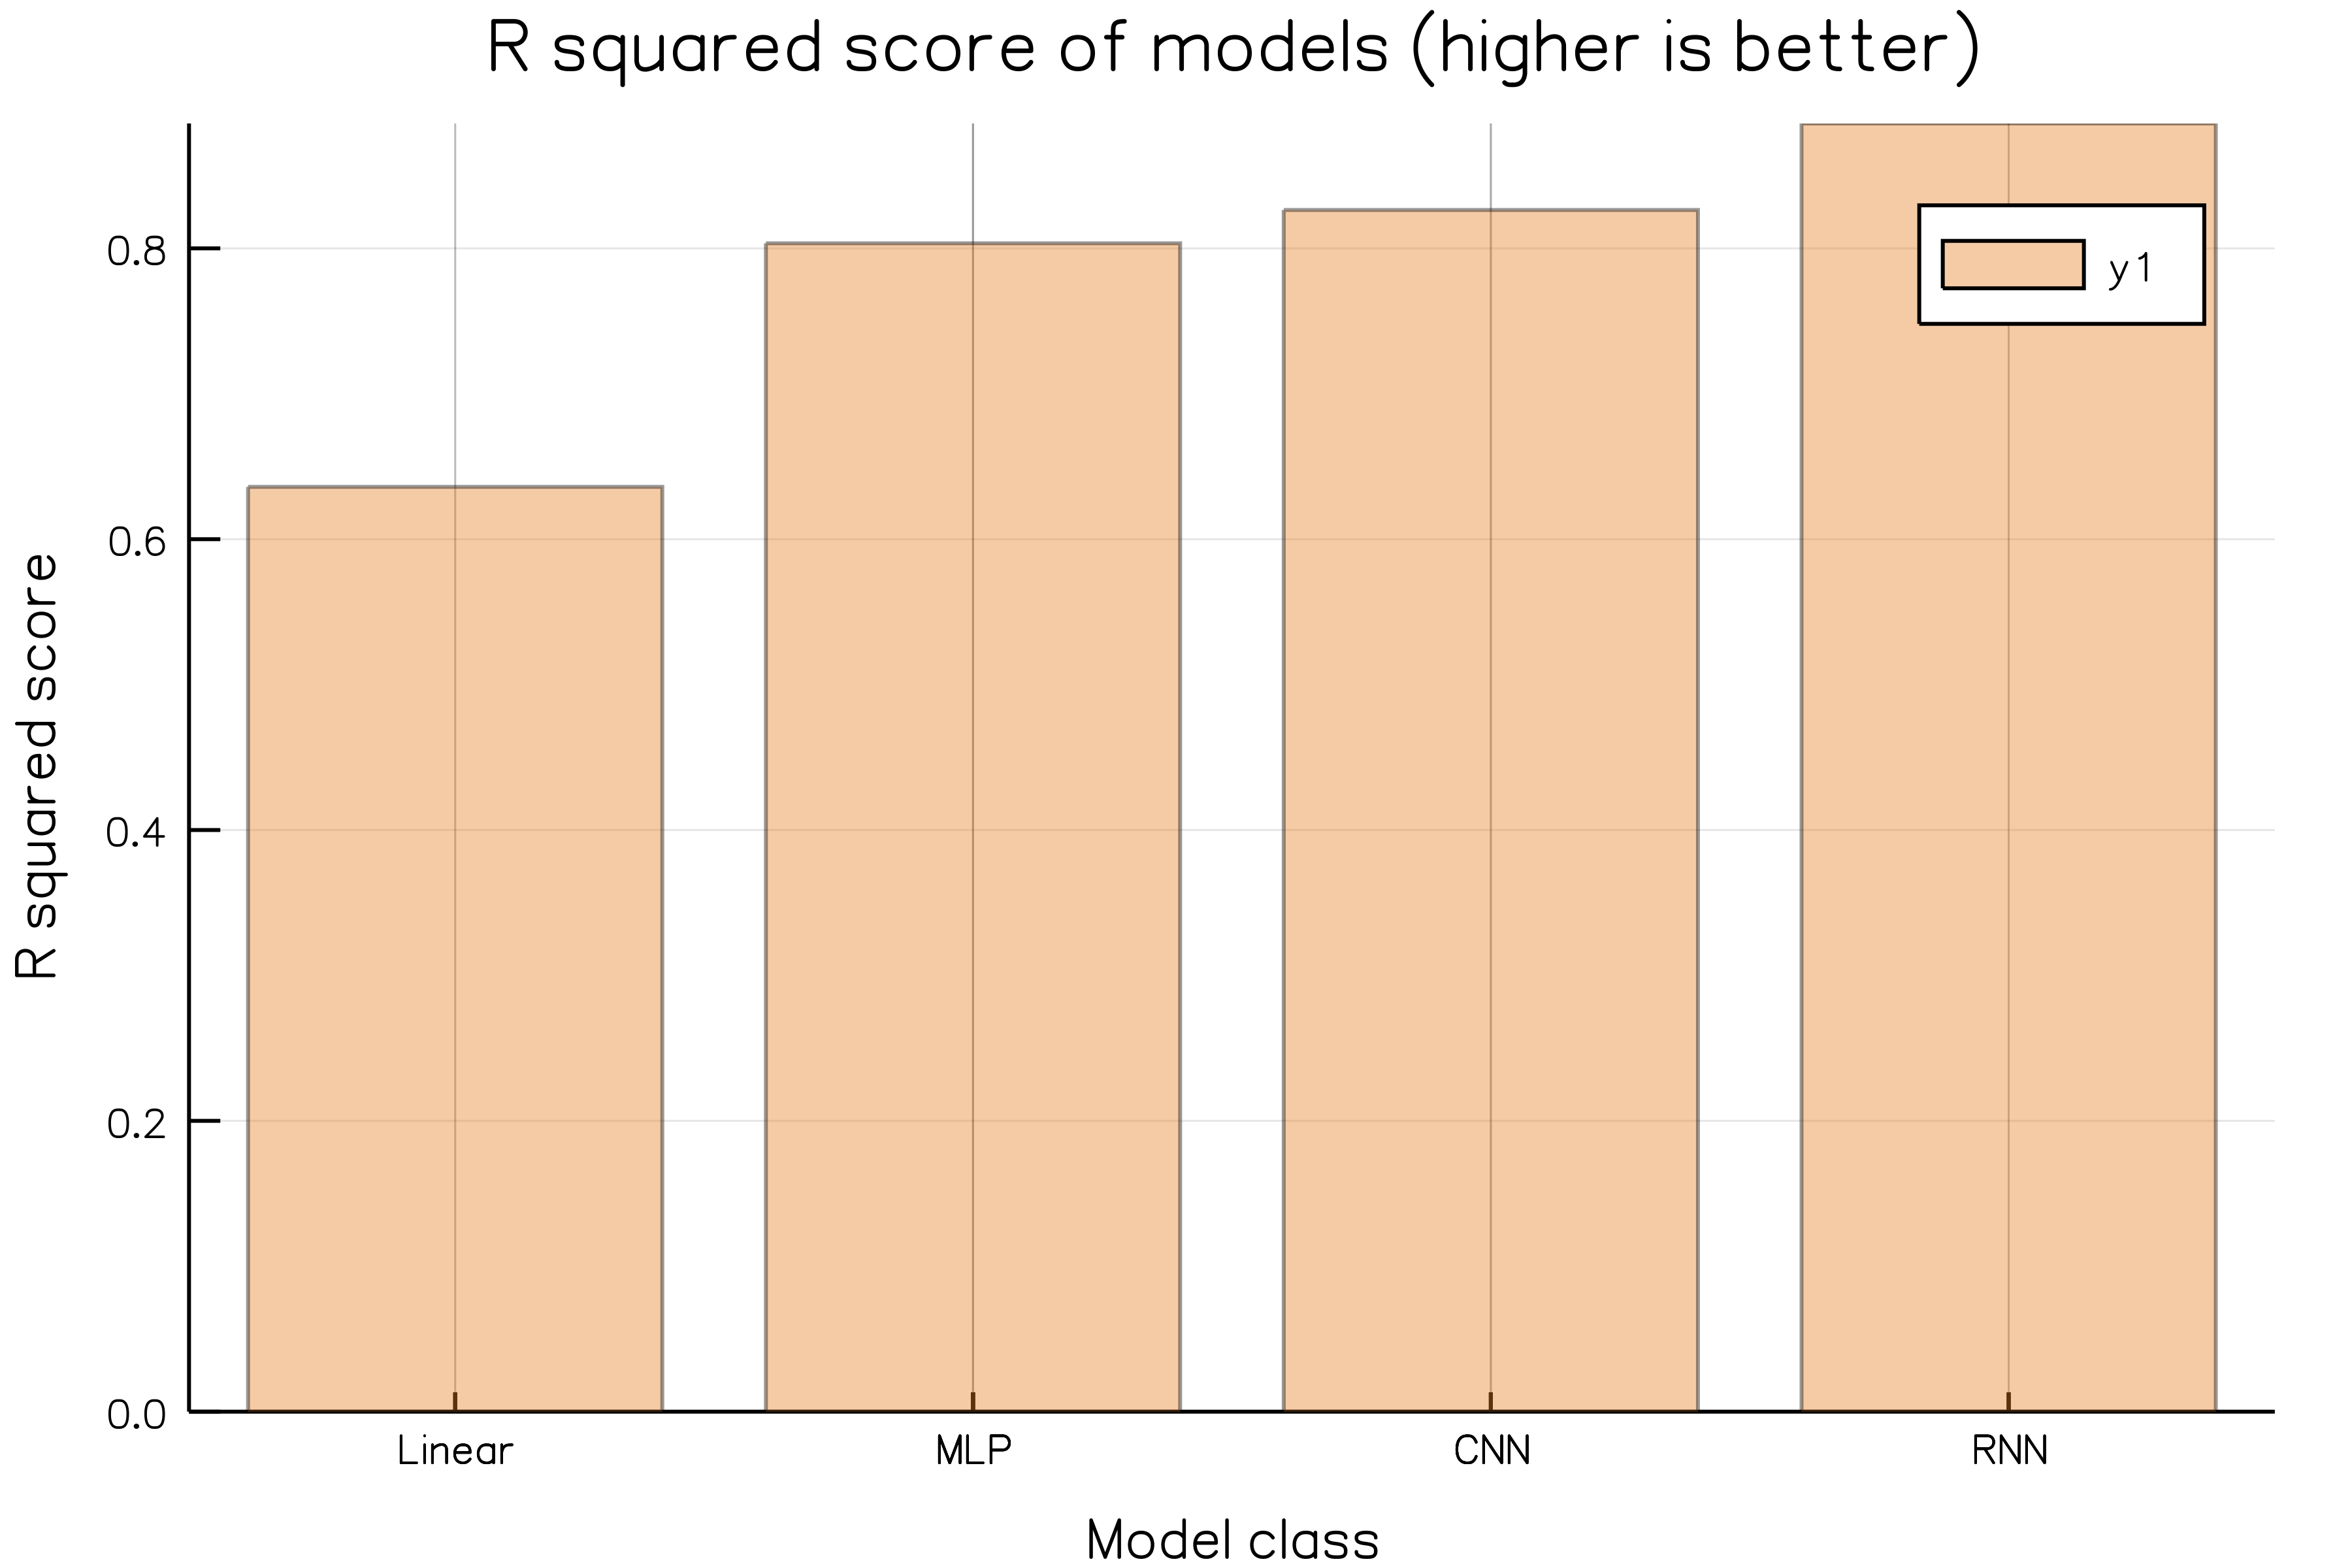
\includegraphics[width=\linewidth]{images/r2_bar.png}
%\vspace{2.4in}
\caption{$R^2$ score across all models}
\label{r2_bar}
\end{figure}
\clearpage
\newpage

\section{Analysis of Strengths and Weaknesses}

In order to fully model a traffic network, the following categories of information must be captured.

\begin{enumerate}
\item Spatially local, temporally local: Information about the bus at the current timepoint, including its location, number of passengers, speed etc.
\item Spatially global, temporally local: Information about the overall traffic network currently, including traffic conditions, number of buses in the network, construction, weather etc.
\item Spatially local, temporally global: Information about each bus which create trends over time, including the bus id, and driver
\item Spatially global, temporally global: Information about the topology of the network overall, including distances between stops, number of intersections, relative location of routes etc.
\end{enumerate}

The linear model can only reason globally, because each input parameter gets one weight.
Therefore no temporal aspects can be captured.

The MLP can do a good job of capturing global data and global trends, so it will be good at modeling numbers 3 and 4.
However it is not really designed for modeling numbers 1 and 2.
Although the input data is inherently a sequence, the MLP treats all inputs equally, so the sequential nature of the data is immediately lost.

Convolutional nets are also able to model number 3 and 4 well, and may be able to capture certain patterns of numbers 1 and 2.
The convolutions respect the sequential nature of the input data, so patterns over time can be captured.
Additionally, CNNs are good at capturing patterns in very high dimensional spaces.
For example, Alpha Go \cite{silver2016mastering} uses a convolutional network to read the Go board and detect similarities between different board positions to create strategies.
Despite the incredible state space of the game of Go, with over $10^170$ possible board positions, the convolutional net can detect which positions are equivalent or similar.
Given access to the entire state of the traffic network, a CNN would do a good job of determining which factors are important for determining travel time.
However this would require an immense amount of training data, because the network has to be able to recognize an immense number of states.
One possible application of CNNs for traffic analysis would be an autoencoder, which takes in the entire state of a traffic network, and extracts the features which are relevant for the prediction task at hand.
This helps reduce the dimensionality of the problem.
However, to truly capture sequential data, RNNs are more suitable.

Compared with the linear, MLP, and CNN models, the RNN is the only one which has state.
This allows it to capture certain properties which the other models cannot.
Recurrent neural networks are well suited to model numbers 1 and 2, and certain types of RNNs can capture numbers 3 and 4.
More specifically, long short term memory networks (LSTMs) do a good job of capturing long term and short term dependencies \cite{hochreiter1997long}.
This makes RNNs the most general model for modeling traffic data, and may explain why they perform the best.
This is because RNNs have memory which is selectively updated based on new data.
In the case of predicting bus arrival times, there is a lot of state which updates over the course of a route.
The number of passengers on the bus, for example, is a quantity which changes over time and is very important in determining how long the bus will stay at each stop.
A feed forward net will not be able to represent this.
This may explain why the RNN performs much better than its feed forward counterparts.
Furthermore, there is a high degree of uncertainty in traffic networks which requires updating your belief of the state based on new information.
RNNs are very well suited for doing this.
In a scenario with free access to all data related to the traffic network, a CNN could be used to distill the entire state into a lower dimensional space.
Then an RNN can be used on the sequential data from each bus to generate accurate predictions based both on the global and local behavior.
